% =====================================================================
%  c07 —— PDF p.55–63（原书 p.49–57）
%  §3.2 稳定图与稳定带状图
%  §3.3 BU(1)^{comb}、EU(1)^{comb} 与基本形式
% =====================================================================

% ===== 原书 p.49 =====
% （本页开头承接 c06 末页延续下来的段落：Coeg 与 S^{an} 的构造，由 c06 译完，
%   此处从略；本块自本页的 \subsection 起译。）
\subsection{稳定图与稳定带状图}

设$(C,p_1,\dots,p_n)$为亏格$g$的$n$点稳定曲线，$V$为$C$的不可约分支的指标集。即设\mbox{$C=\bigcup_{v\in V}C_v$}。定义$V_c$及$V_{nc}$为
\[
\begin{aligned}
V_c&=\{v\in V\mid C_v\text{上没有任何标记点}\},\\
V_{nc}&=\{v\in V\mid C_v\text{上至少有一个标记点}\}.
\end{aligned}
\]

% ===== 原书 p.50 =====
并定义：当$v$为$V_c$或$V_{nc}$的元素时，分别称$C_v$为紧分支或非紧分支。

以$Q$为奇点集的指标集，设$r_1,\dots,r_n\in\R_+$。当$v$为$V_{nc}$的元素时，作为前一章二次微分存在定理的极限，$C_v$上存在亚纯二次微分$\omega_v$。即，取$p_1,\dots,p_m$为$C_v$的标记点、$q_1,\dots,q_m$为$C_v$的奇点，把$\omega_v(r_1,\dots,r_m,\varepsilon_1,\dots,\varepsilon_l)$取作在$p_1,\dots,p_m,q_1,\dots,q_l$周围具有长为$r_1,\dots,r_m,\varepsilon_1,\dots,\varepsilon_l$的闭轨道的二次微分，并把极限
\[
\lim_{\varepsilon_i\to0}\omega_v(r_1,\dots,r_m,\varepsilon_1,\dots,\varepsilon_l)
\]
记作$\omega_v$。

\transnote{原文此句前半印作「$q_1,\dots,q_m$ を $C_v$ の singular point として」，同一句稍后又写作$q_1,\dots,q_l$，下文亦一律用$q_l$；据上下文，前半似应为$q_l$。此处照原文印出。}

\begin{enumerate}[label=(\arabic*)]
\item 设$p_i$位于$C_v$上，$p_i$处的局部坐标为$z_i$，则$\omega_v$局部地写作
\[
\omega_v=\Bigl(\frac{r_i^2}{z_i^2}+O\Bigl(\frac{1}{z_i}\Bigr)\Bigr)dz_i^{\otimes2}.
\]
\item 设$q_i$为位于$C_v$上的奇点，则$\omega_v$局部地写作
\[
\omega_v=O\Bigl(\frac{1}{z_i}\Bigr)dz_i^{\otimes2}.
\]
\item $\omega_v$在$p_1,\dots,p_m,q_1,\dots,q_l$以外全纯。
\item 它具有闭轨道，其特征环域与绕$p_1,\dots,p_m$的小环同伦等价。又，任何特征环域的内部都不含$q_1,\dots,q_l$。
\end{enumerate}

由此在各$C_v$上构成带状图$G(v)$，$G(v)$具有以下性质。
\begin{enumerate}[label=(\arabic*)]
\item $G(v)$的顶点有两类：二次微分的绝对值$|\omega_v|$的临界点$K_v$与奇点$Q_v$。
\item $q\in Q_v$的价数$v(q)$不小于$1$，$p\in K_v$的价数不小于$3$。
\item 设$C_v$的亏格为$g(v)$，则作为带状图的边界有$m$个，$G(v)$的 Euler–Poincaré 示性数为$2-2g(v)-m$。
\end{enumerate}

% ===== 原书 p.51 =====
又，把这个边界的个数记作$m(v)$、$Q_v$的个数记作$l(v)$。对于这样的带状图，即给定两类顶点、$\#Q=l$、边界个数为$m$，设其 Euler–Poincaré 示性数为$\chi(G)$，令$g=\frac12(2-\chi(G)-m)$，称$G$为类型$(g,l,m)$的带状图。

又，给定亏格$g$的$n$点稳定曲线$C$时，把它的分支用点表示、把相交用连接对应分支之点的线表示，如此定义的图，即$C$的对偶图$\Gamma$。此时对每个点$v$赋予对应曲线的亏格$g(v)$这一数据。进而对应于标记点，从表示分支的点引出、不与其他任何点相连的线，即外棱与之对应。此时图$\Gamma$具有以下性质。
\begin{enumerate}[label=(\arabic*)]
\item $g=\sum_{n}g(v)+\rank_{\Z}(H^1(\Gamma,\Z))$
\item $\Gamma$中总共有$n$条外棱。
\item 由$g(v)=0$构成的顶点（把外棱也算在内）至少引出$3$条线。
\end{enumerate}

\transnote{第 (1) 条的下标原文印作$\sum_{n}$，按文意应是对顶点$v$求和$\sum_{v}$；此处照原文译出。}

具有上述 (1)～(3) 性质的连通图，连同其顶点上的数据$\{g(v)\}_v$，称为类型$(g,n)$的对偶图。对偶图$\Gamma$的非紧分支，是指至少引出一条外棱的顶点。非紧分支的集合记作$V_{nc}$。对$v\in V_{nc}$，定义
\[
l(v)=\#\{\,\text{边}\mid v\text{为其一个端点}\,\}
\]
（两端都为$v$的边计作两条。）
\[
m(v)=\#\{\,\text{外棱}\mid\text{从}v\text{引出}\,\}.
\]

对偶图$\Gamma$及其非紧分支$v\in V_{nc}$，给定了类型$(g(v),m(v),l(v))$的带状图的对象$(\Gamma,G(v),(v\in V_{nc}))$，称为类型$(g,n)$的稳定带状图。类型$(g,n)$的稳定带状图的全体记作$\widetilde{S}_{g,n}$。又，稳定带状图连同其边界（共有$n$个）上沿自然定向的标架，称为带标架的稳定带状图，其全体记作$\widetilde{FS}_{g,n}$。这里所谓的沿自然定向的标架，例如是下面那样的标架。

% ===== 原书 p.52 =====
\begin{center}
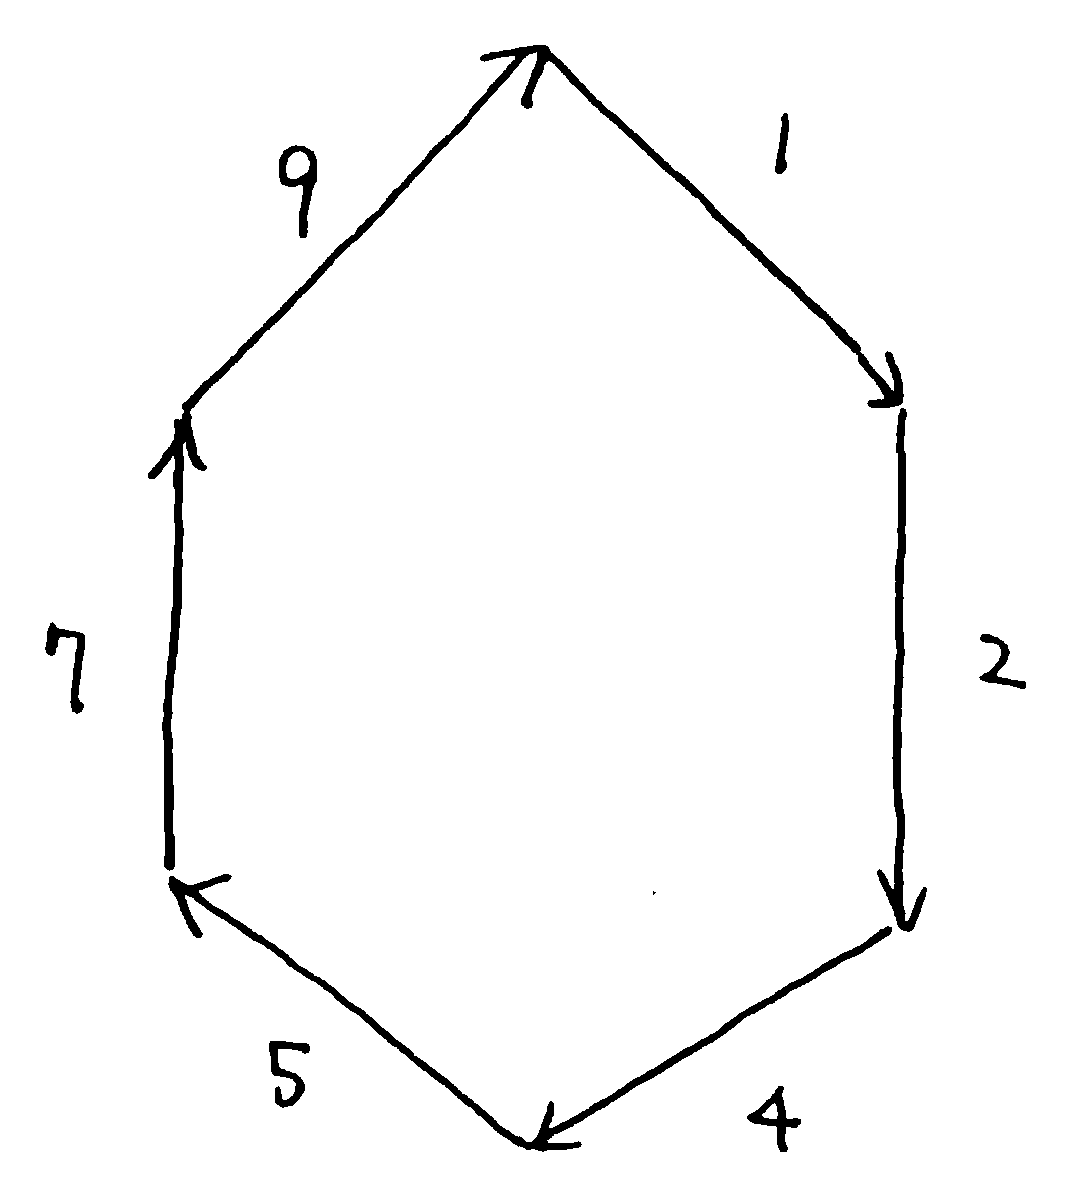
\includegraphics[width=5.0cm]{fig_p58_a.png}
\end{center}

给$\widetilde{FS}_{g,n}$的每条边赋以长度，所得的称为带度量的带标架稳定带状图，其全体记作$\widetilde{MFS}_{g,n}$。在$\widetilde{MFS}_{g,n}$中，忘掉度量信息后得到给定的$(\Gamma,G(v))\in\widetilde{FS}_{g,n}$的全体，因边界上带有标架，自然地同一视作$\R_+^a$。这里$a$是$G(v)$（$v\in V_{nc}$遍历）的边的总数。

下面定义某种等价关系。设$(\Gamma,G(v)),(\Gamma',G'(v))$为$\widetilde{S}_{g,n}$的两个元素。把$\Gamma$中以$k$条边相连的分支$v_1,v_2$替换为$v_3$，令$g(v_3)=g(v_1)+g(v_2)+(k-1)$，设由此得到$\Gamma'$。例如下图那样的替换。
\begin{center}
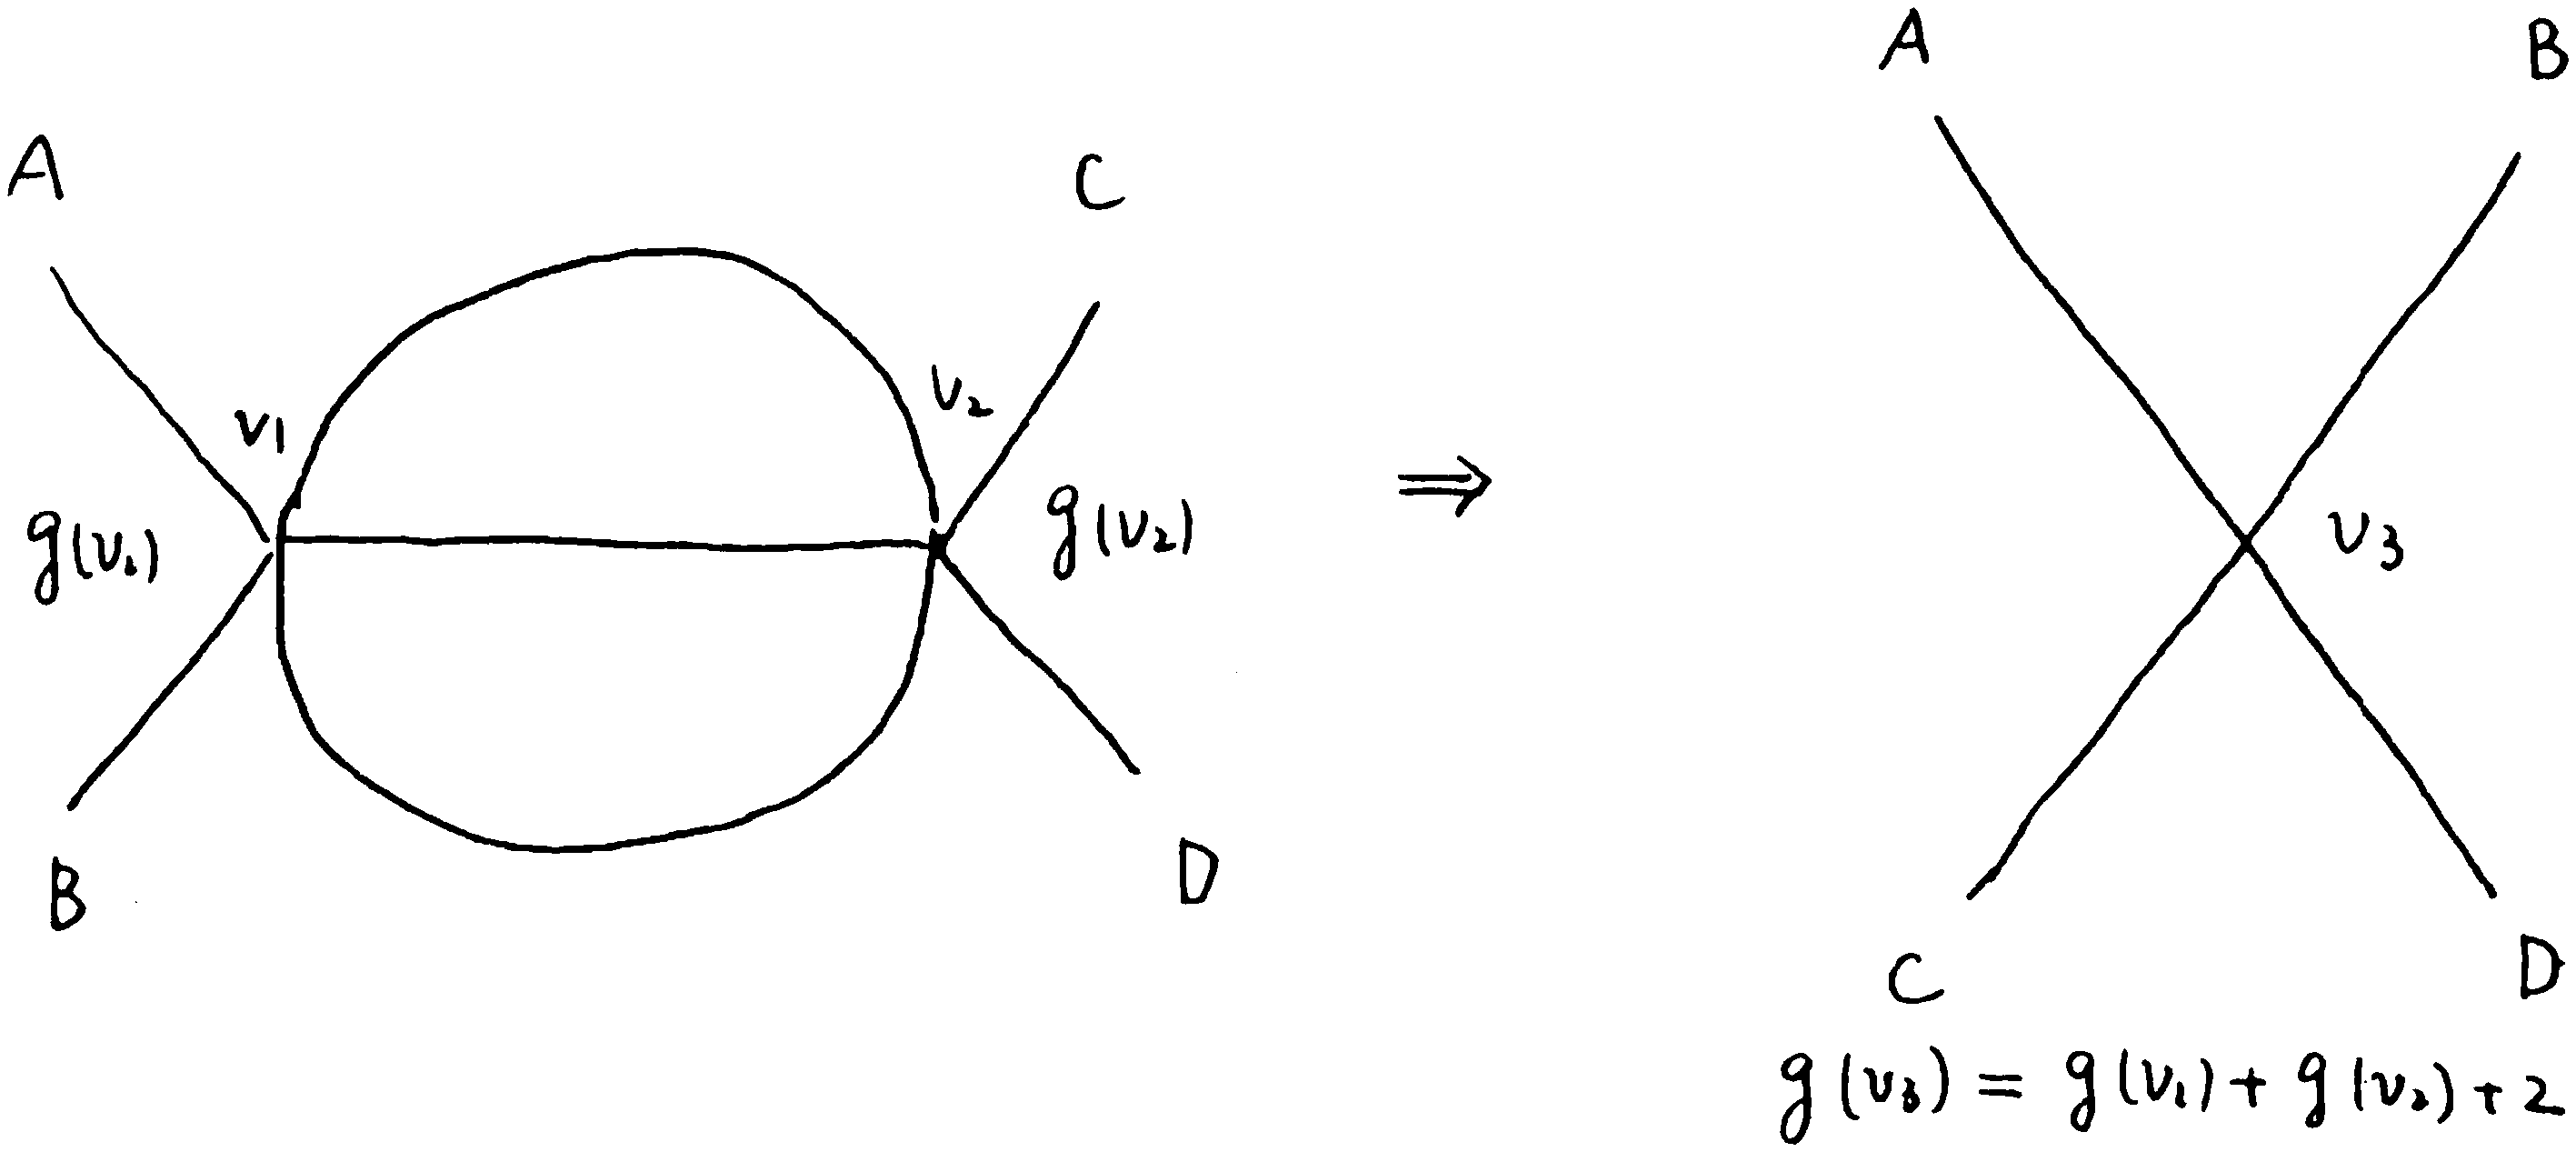
\includegraphics[width=11cm]{fig_p58_b.png}
\end{center}

此时$\Gamma,\Gamma'$的$V_{nc}$没有任何变化，故在等同视之时，设$G(v),G'(v)$作为带状图同构。

% ===== 原书 p.53 =====
考虑使这样的$(\Gamma,G(v))$与$(\Gamma',G'(v))$等价的等价关系。例如下面两个是等价的。
\begin{center}
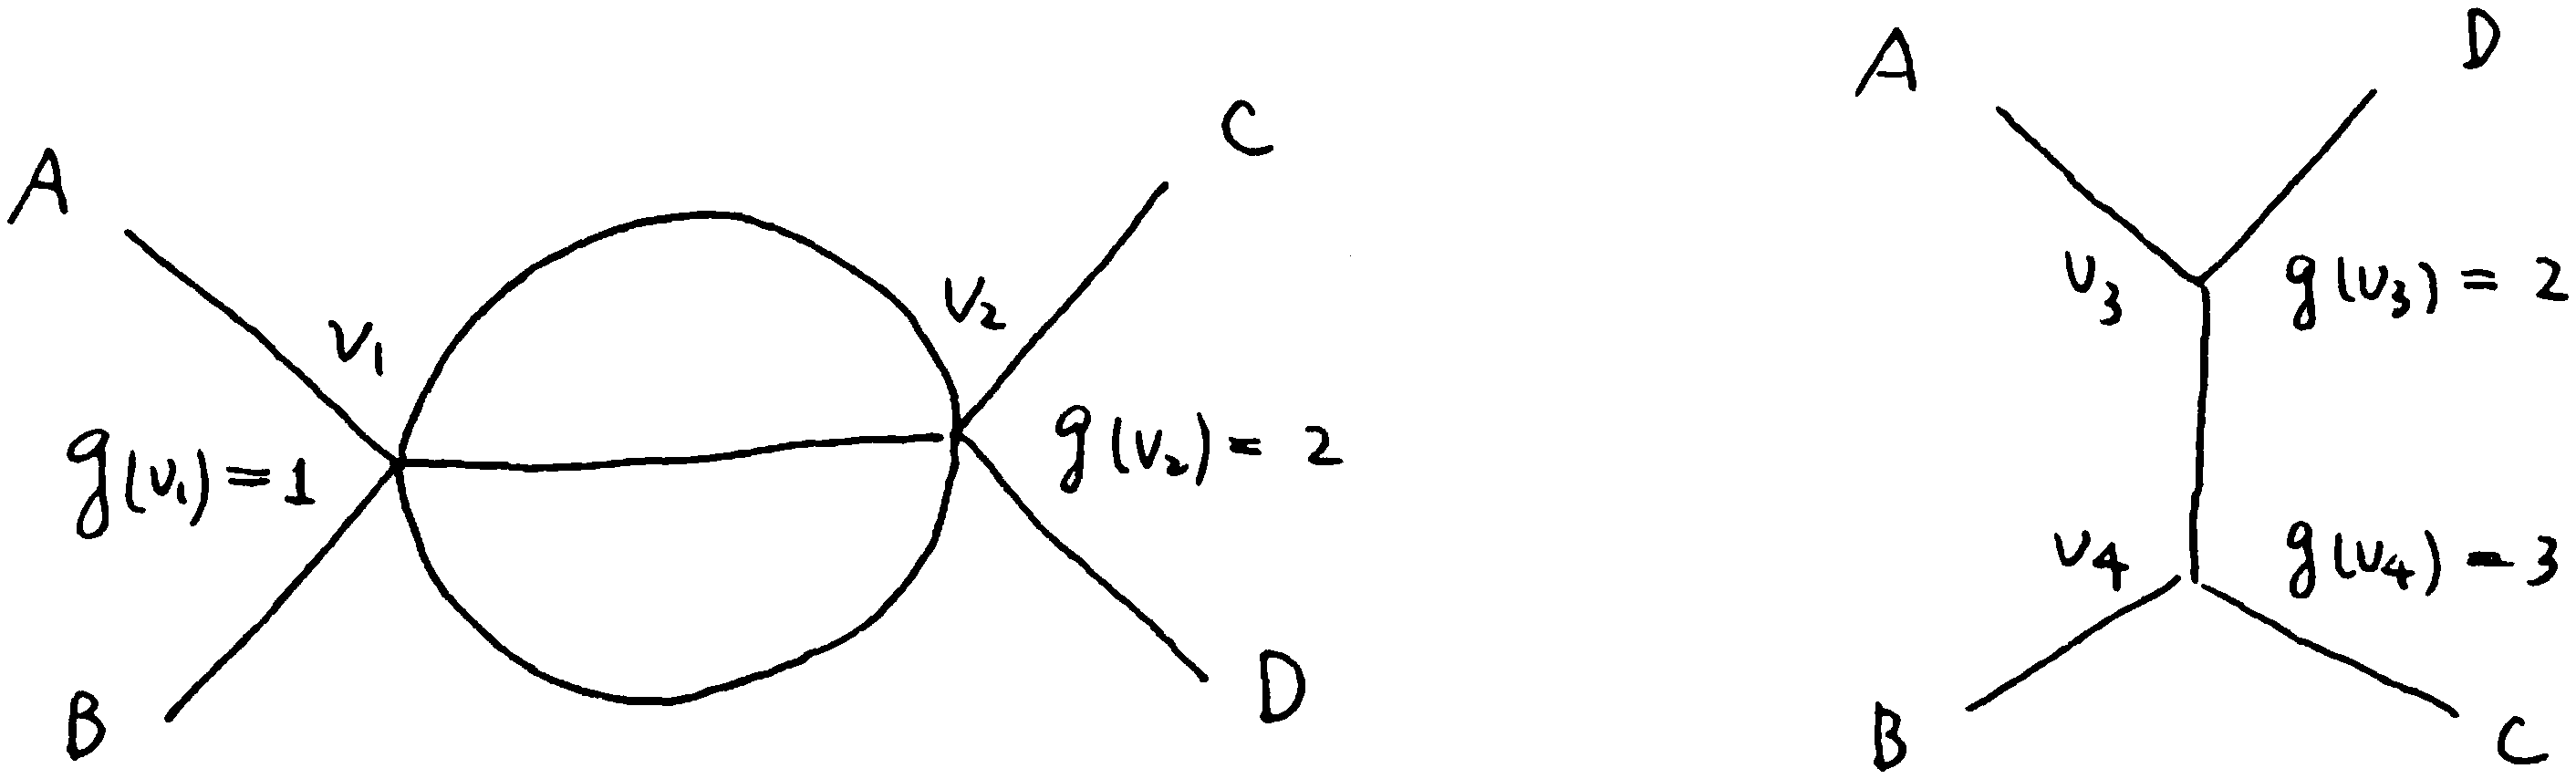
\includegraphics[width=10.5cm]{fig_p59_a.png}
\end{center}

把这个等价关系下的商空间$\widetilde{S}_{g,n}/\!\sim$定义为$S_{g,n}$。在上面的$G(v)$与$G'(v)$同构之处，按连边界的命名也算在内而同构，由此引入$\widetilde{FS}_{g,n}$上的等价关系，其商空间记作$FS_{g,n}=\widetilde{FS}_{g,n}/\!\sim$。进一步，按连度量也保持下来引入$\widetilde{MFS}_{g,n}$上的等价关系，其商空间$\widetilde{MFS}_{g,n}/\!\sim$记作$MFS_{g,n}$。此时$MFS_{g,n}$是以$(\Gamma,G(v))\in FS_{g,n}$为指标集的一族形如$\R_+^a$的空间的无交并。这里$a$如前所述，是$G(v)$（$v\in V_{nc}$）中出现的边的总数。在其上引入由度量退化而来的自然拓扑。度量退化时也会从$G(v)$生出紧分支，故为慎重起见记下其方法。例如考虑把下面的$A$与$B$粘贴所得的带状图。
\begin{center}
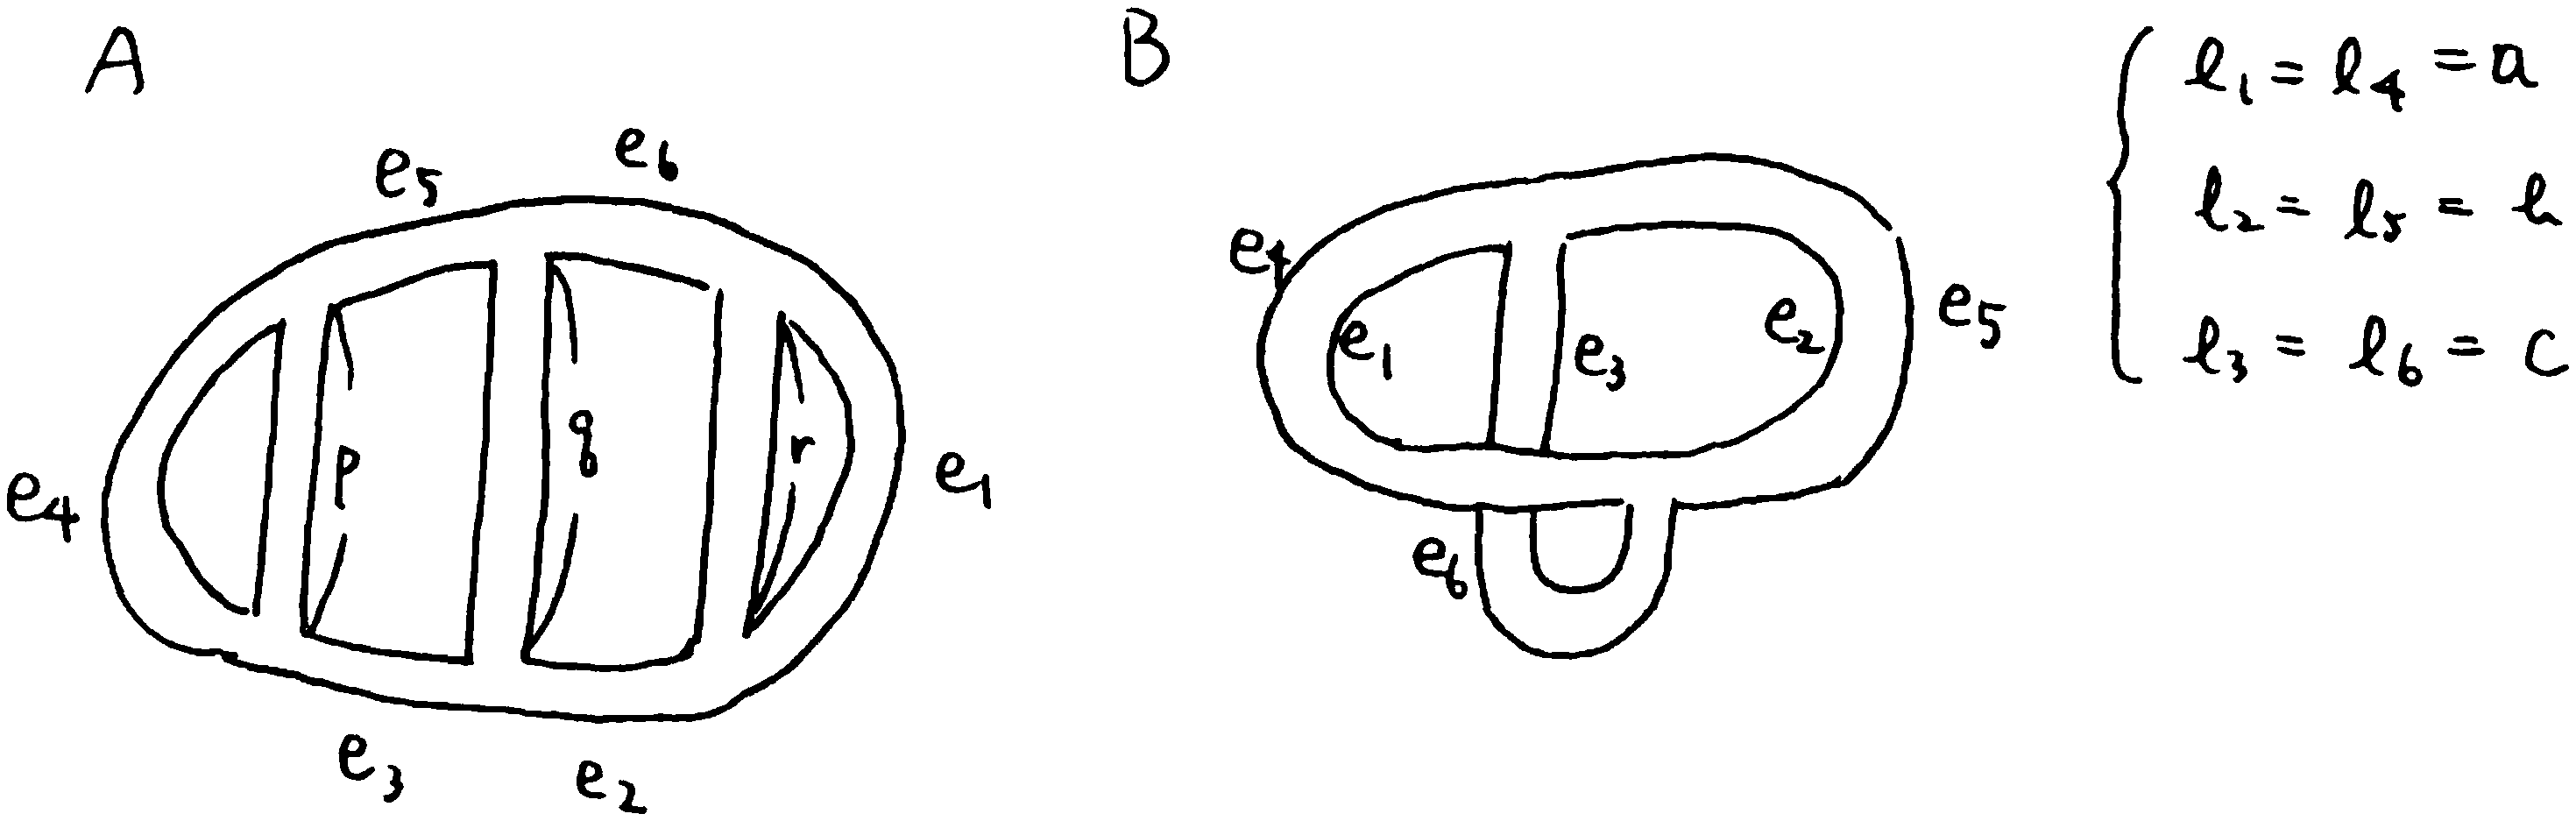
\includegraphics[width=11cm]{fig_p59_b.png}
\end{center}

这里$A$与$B$按$1\sim6$同号相粘贴，各自的长度由$a,b,c$给出。分别固定$p>0,q>0,r>0$不变而令$a+b+c\to0$时，从$B$得到亏格$1$的曲线。从$A$得到被标记$4$个点、其中$1$点为奇点的亏格$0$曲线。$A$的边界长度如图所见，收敛于$p,p+q,p+r,r$。此时亏格$0$的分支退化如下面 (c) 那样的带状图。

% ===== 原书 p.54 =====
\begin{center}
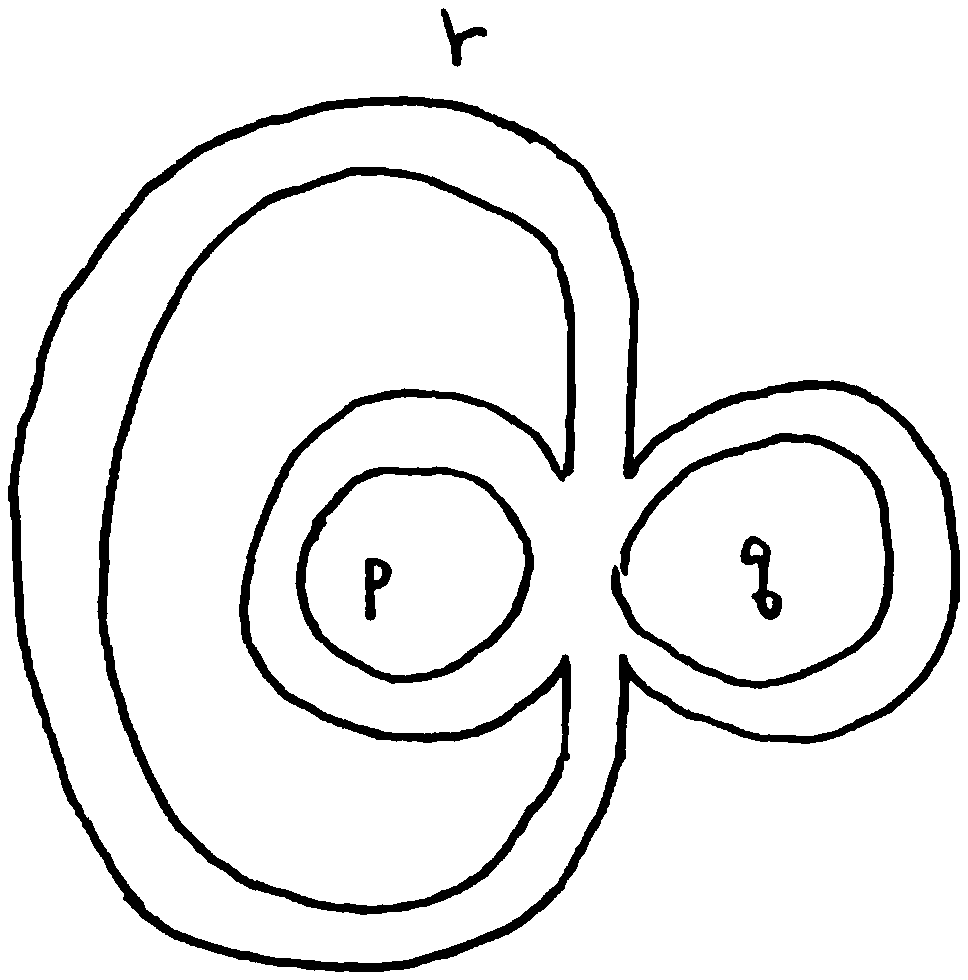
\includegraphics[width=4.5cm]{fig_p60_a.png}
\end{center}

此时，把$\R_+^6=\{(a,b,c,p,q,r)\}$与$\R_+^3=\{(0,0,0,p,q,r)\}$的并看作$\R_{\ge0}^6$，以诱导拓扑赋予拓扑。如此，$MFS_{g,n}$上就有了自然的拓扑。

又设$(\Gamma_1,G_1(v)),(\Gamma_2,G_2(v))\in MNS_{g,n}$。当忘掉$G_1(v),G_2(v)$边界上的标架后同构时，称它们作为带度量的稳定带状图同构。（这里总考虑保持边界编号的映射。）令$(\Mbar^{comb}_{g,n})_0=MFS_{g,n}$，并定义
\[
\begin{aligned}
(\Mbar^{comb}_{g,n})_1=\bigl\{&(a,b,\phi:a\rightleftarrows b)\ \bigm|\ a,b\in(\Mbar^{comb}_{g,n})_0,\\
&\phi\text{是作为带度量带状图的同构}\bigr\}.
\end{aligned}
\]

\transnote{这里写$MNS_{g,n}$，与前面定义的$MFS_{g,n}$不一致，疑为$MFS_{g,n}$之误；此处照原文译出。}

此时自然的投影$\mathrm{pr}_i$（$i=1,2$）如下定义。
\[
\begin{aligned}
(\Mbar^{comb}_{g,n})_1\ni(a,b,\phi)&\overset{\mathrm{pr}_1}{\longmapsto}a\in(\Mbar^{comb}_{g,n})_0,\\
(\Mbar^{comb}_{g,n})_1\ni(a,b,\phi)&\overset{\mathrm{pr}_2}{\longmapsto}b\in(\Mbar^{comb}_{g,n})_0.
\end{aligned}
\]

这里$\mathrm{pr}_1,\mathrm{pr}_2$遗憾地不是局部同构，但像前一章那样，令
\[
\begin{aligned}
(\Mbar^{comb}_{g,n})_k={}&(\Mbar^{comb}_{g,n})_1\times_{(\Mbar^{comb}_{g,n})_0}\cdots\\
&\times_{(\Mbar^{comb}_{g,n})_0}(\Mbar^{comb}_{g,n})_1\qquad(\text{$k$个}),
\end{aligned}
\]
构成分片线性空间的单纯对象。

\begin{definition}
\[
\Mbar^{comb}_{g,n}=\Coeq\bigl((\Mbar^{comb}_{g,n})_1\rightrightarrows(\Mbar^{comb}_{g,n})_0\bigr).
\]
又，用单纯空间$\{(\Mbar^{comb}_{g,n})_k\}_{k\ge0}$来定义$H^*(\Mbar^{comb}_{g,n},\Q)$。
\end{definition}

% ===== 原书 p.55 =====
\subsection{$BU(1)^{comb}$、$EU(1)^{comb}$与基本形式}

把空间$(BU(1)^{comb})_0$用$\varinjlim_{N}(\R_{\ge0}^N-\{0\})$定义。这里$\R_{\ge0}^N-\{0\}\to\R_{\ge0}^{N+1}-\{0\}$由$(a_1,\dots,a_N)\mapsto(a_1,\dots,a_N,0)$定义。

设$a=(a_1,\dots,a_N)\in(BU(1)^{comb})_0$。把$a_i\neq0$的$i$依次记作$a_{i_1},\dots,a_{i_m}$，考虑名为$e_{i_k}$、长度由$a_{i_k}$给出的边的环，由此对应以带度量的带基点的环。

\transnote{原文此处把满足$a_i\neq0$的下标$i$依次记作$a_{i_1},\dots,a_{i_m}$，混用了下标与分量，疑应为$i_1,\dots,i_m$；此处照原文译出。}

\begin{center}
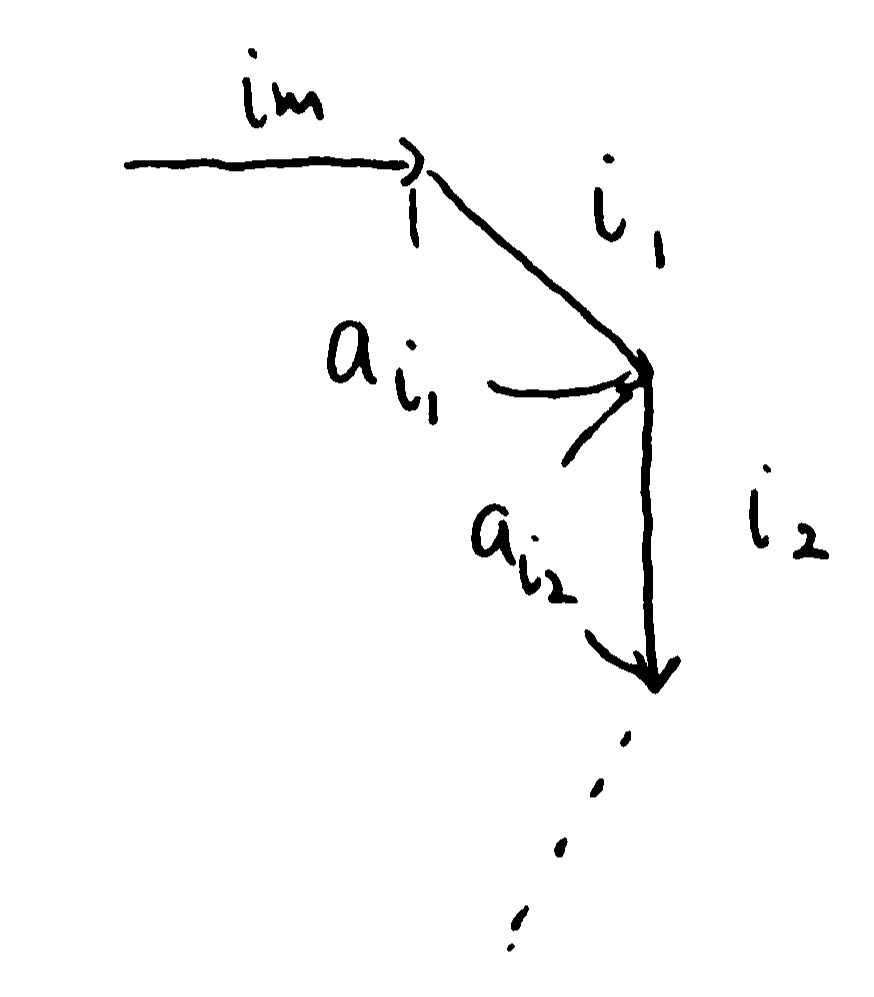
\includegraphics[width=4.0cm]{fig_p61_a.png}
\end{center}

$a,b$作为带度量的环同构，是指由$a$经重编号与重取基点得到$b$。此时把这个替换记作$\phi:a\to b$。例如取$a=(1,1,0,0)$、$b=(0,1,0,1)$，则凑巧两者长度都为$1$，故$\Hom(a,b)$是二元集合$\{\phi_1,\phi_2\}$。这里
\[
\phi_1:e_1\to e_2,\quad e_2\to e_3,\qquad
\phi_2:e_1\to e_3,\quad e_2\to e_2.
\]

\begin{center}
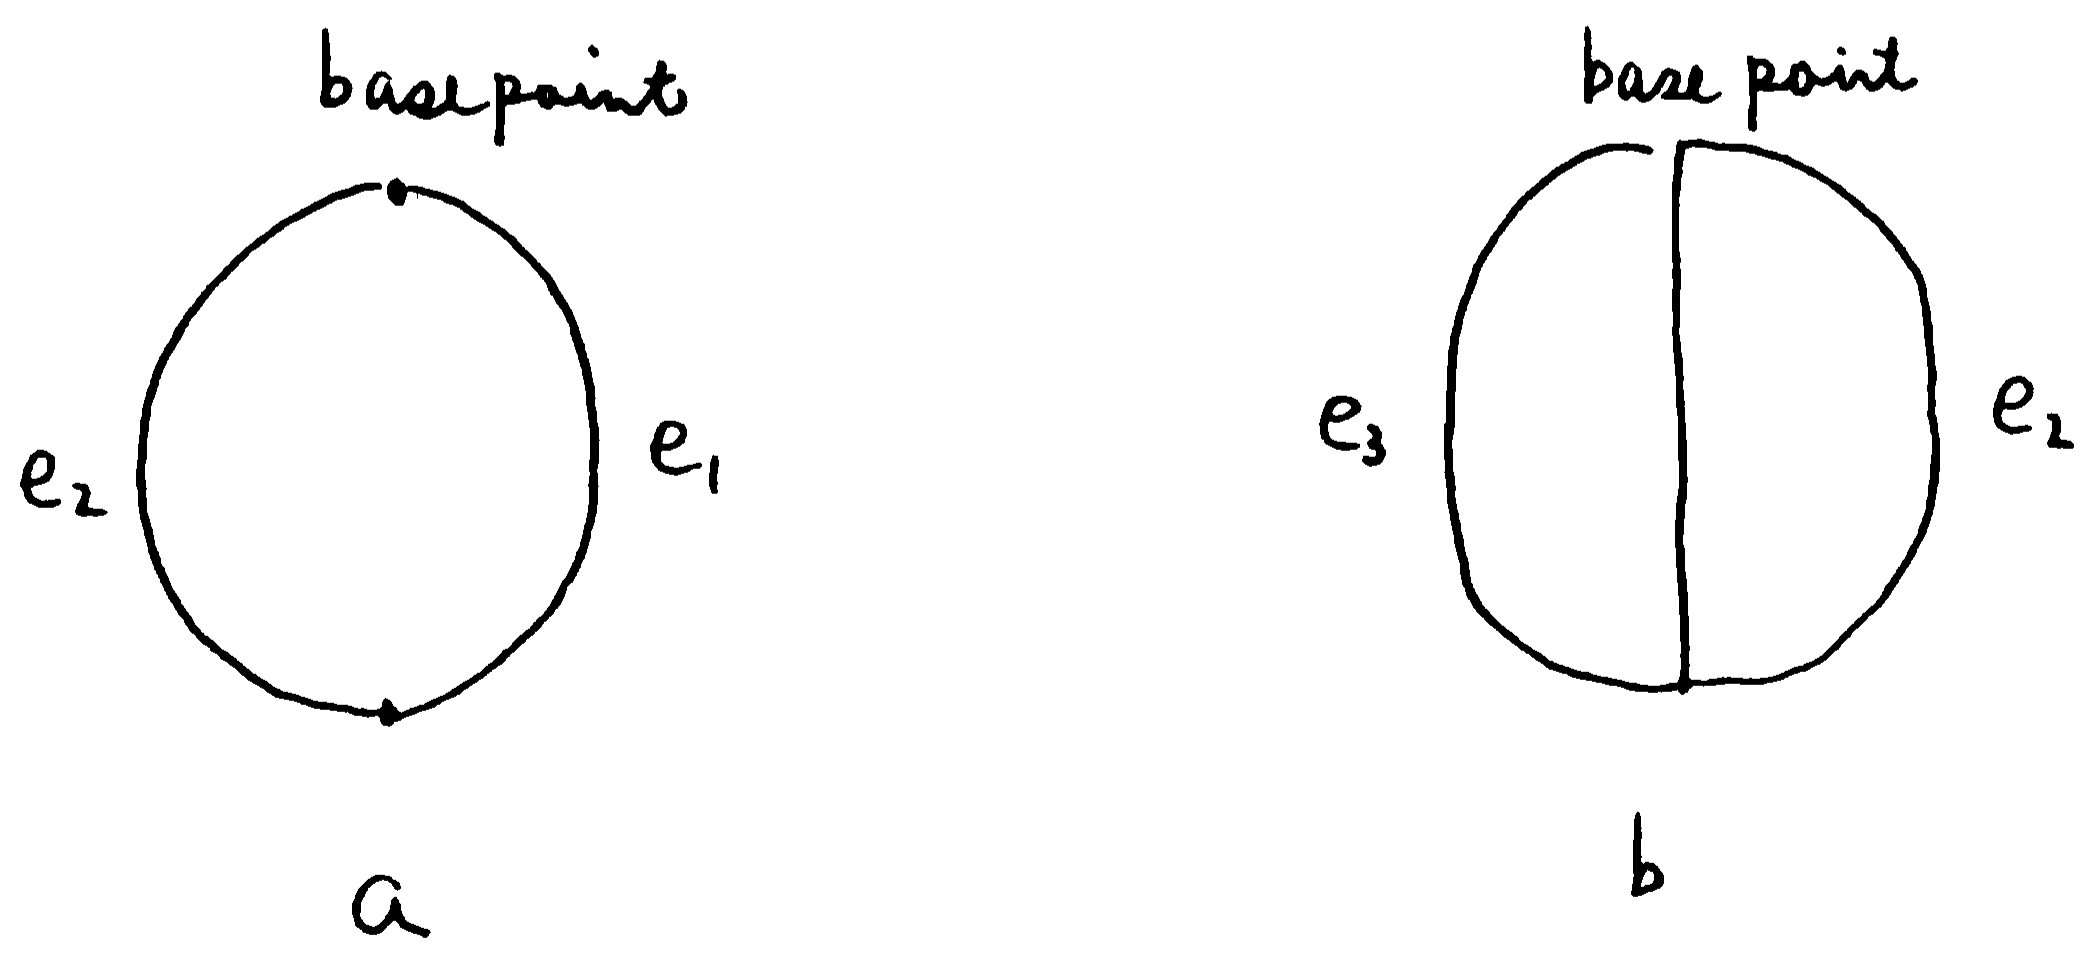
\includegraphics[width=8.5cm]{fig_p61_b.png}
\end{center}

\transnote{原文取$b=(0,1,0,1)$，其非零分量对应$e_2,e_4$，而上面的$\phi_1,\phi_2$却用到$e_3$，图 (b) 也标作$e_3,e_2$；原文前后不一致，疑$b=(0,1,1,0)$或$\phi$中应为$e_4$；此处照原文译出。}

\[
\begin{aligned}
(BU(1)^{comb})_1=\bigl\{&(a,b,\phi)\ \bigm|\ a,b\in(BU(1)^{comb})_0,\\
&\phi:a\to b\text{是作为带度量的环的同构}\bigr\}.
\end{aligned}
\]

% ===== 原书 p.56 =====
这样置定。前面所述的理由表明$\mathrm{pr}_i:(BU(1)^{comb})_1\to(BU(1)^{comb})_0$不是局部同构，但可构成分片线性单纯对象$\{(BU(1)^{comb})_k\}_k$。

\begin{definition}
\[
BU(1)^{comb}=\Coeq\bigl((BU(1)^{comb})_1\rightrightarrows(BU(1)^{comb})_0\bigr).
\]
\end{definition}

下面构成$BU(1)^{comb}$上的万有$S^1$丛$EU(1)^{comb}$。
\[
\begin{aligned}
(EU(1)^{comb})_0&=\{(a,p)\mid a\in BU(1)^{comb},\ p\in a\},\\
(EU(1)^{comb})_1&=\{(a,b,\phi,p)\mid(a,b,\phi)\in(BU(1)^{comb})_1,\ p\in a\}.
\end{aligned}
\]

此时，$(EU(1)^{comb})_1\to(EU(1)^{comb})_0\times(EU(1)^{comb})_0$是单射，其像给出$(EU(1)^{comb})$上的等价关系。把这个等价关系下的商空间$(EU(1)^{comb})_0/\!\sim$中对应多边形$a$的边数恰好为$N$的部分记作$EU(1)^{comb}_N$，则它与下面的空间同一视。
\[
\begin{aligned}
\bigl\{(r,\phi_1,\dots,\phi_N)\ \bigm|\ &r\in\R_+,\ \phi_i\in\R/r\Z,\ \phi_i\neq\phi_{i+1},\\
&\phi_i\text{沿环排列},\ \phi_N\le0<\phi_1\bigr\}.
\end{aligned}
\]

在这个空间上取局部坐标$(r,\tilde\phi_1,\dots,\tilde\phi_N)$。这里$\tilde\phi_i\in\R$是$\phi_i$在$\R$中的代表元。此时$d(\tilde\phi_i/r)$不依赖坐标的取法，故记作$d(\phi_i/r)$。取满足$l_i\equiv\phi_{i+1}-\phi_i\bmod r\Z$、$0\le l_i<r$的函数$l_i$，用它定义$EU(1)^{comb}_N$上的$1$次形式
\[
\alpha=\sum_{i=1}^{N}\frac{l_N}{r}\wedge d\Bigl(\frac{\phi_i}{r}\Bigr).
\]

\transnote{上式第$i$项的系数原文印作$l_N/r$，与随后对$d\alpha$的计算及各系数$l_1,\dots,l_N$不符，疑应为$l_i/r$；此处照原文译出。}

现固定$l_1,\dots,l_N>0$，置
\[
\begin{aligned}
S^1(l_1,\dots,l_N)=\bigl\{(r,\phi_1,\dots,\phi_N)\in EU(1)^{comb}_N\ \bigm|\ &r=l_1+\cdots+l_N,\\
&l_i\equiv\phi_{i+1}-\phi_i\ (\mathrm{mod}\ r\Z)\bigr\}.
\end{aligned}
\]

% ===== 原书 p.57 =====
则$\int_{S^1(l_1,\dots,l_N)}\alpha=-1$。按下图作坐标变换$(r,\phi_1,\dots,\phi_N)\mapsto(l_1,\dots,l_N,t)$（$0\le t<l_N$）：
\[
\phi_1=l_N-t,\qquad \phi_2=l_1+l_N-t,\ \dots
\]
\begin{center}
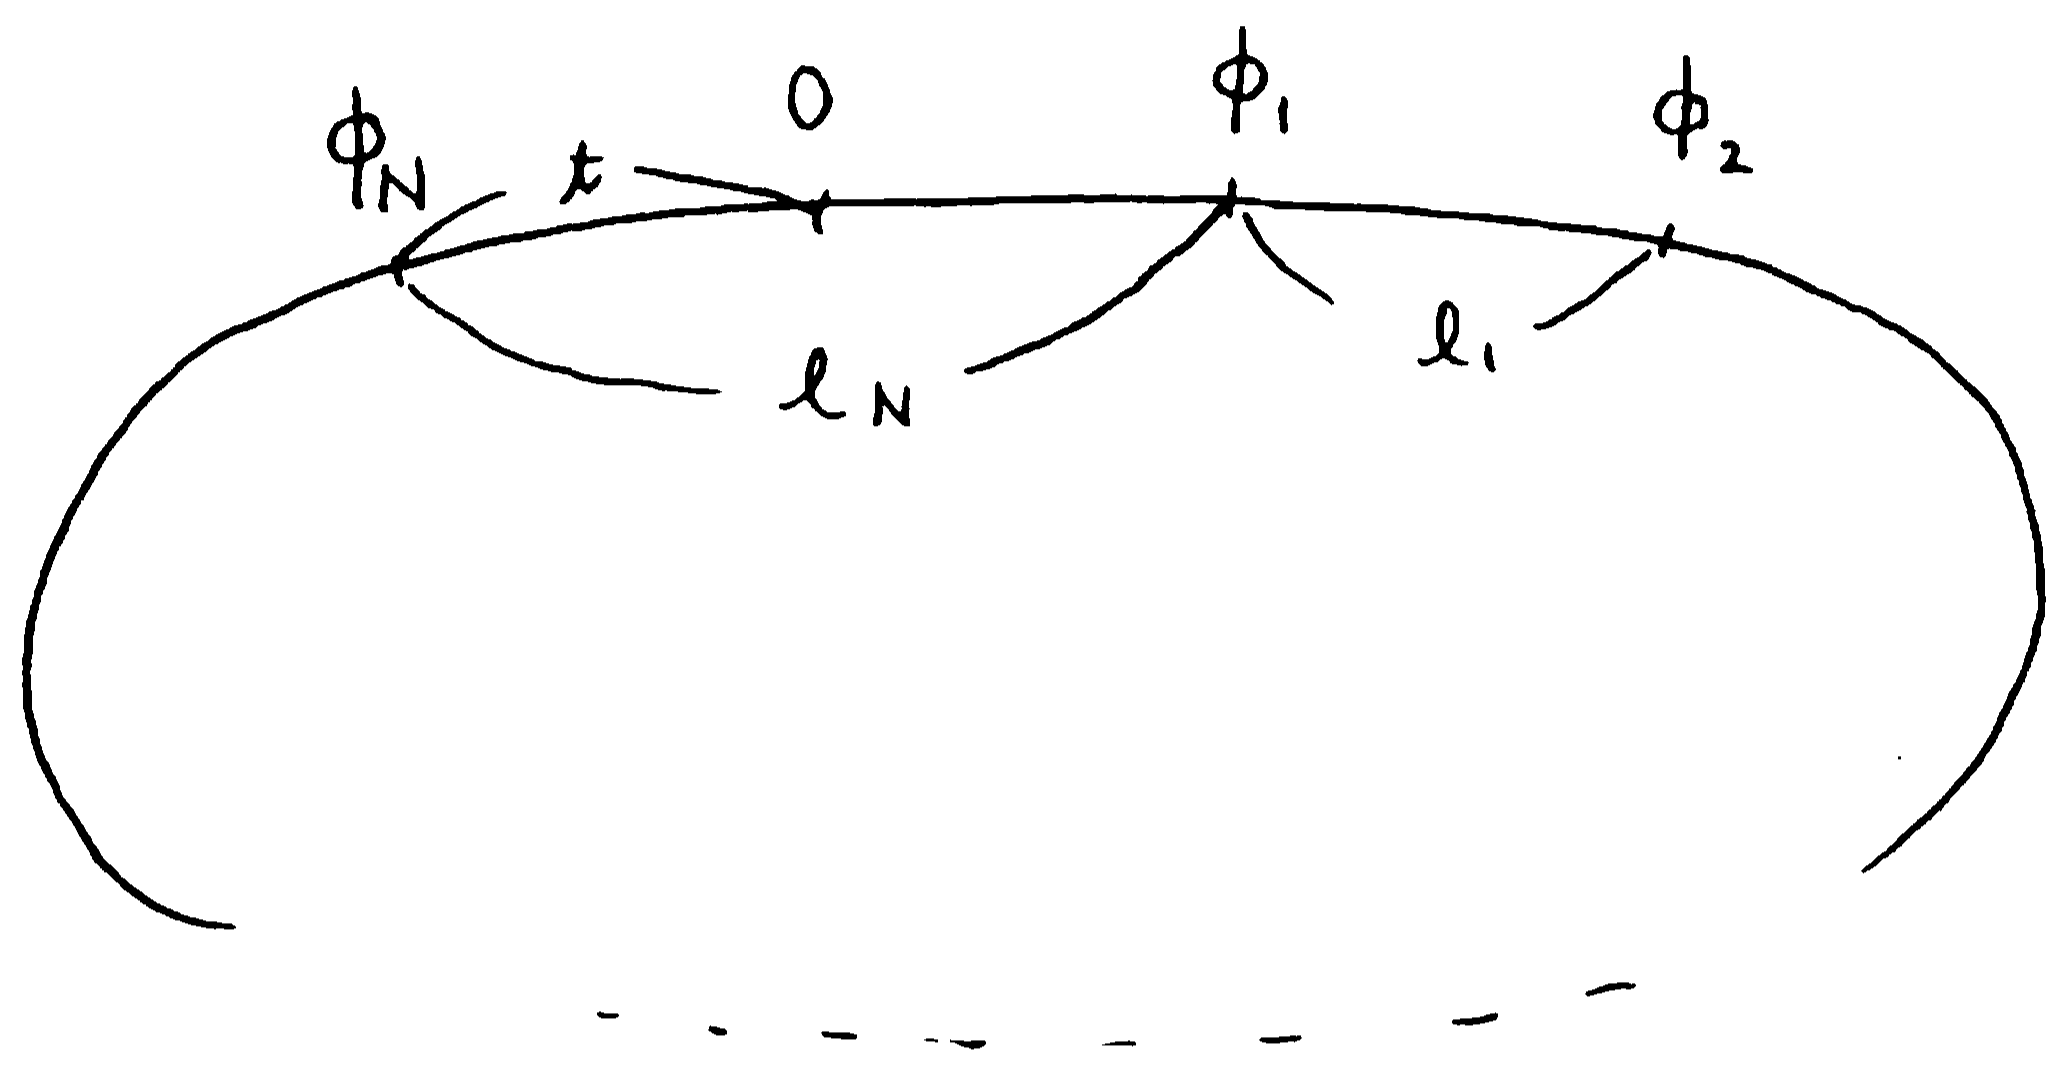
\includegraphics[width=8.0cm]{fig_p63_a.png}
\end{center}

此时，$\alpha$表示为
\[
\begin{aligned}
\alpha&=\frac{l_1}{r}\wedge d\Bigl(\frac{l_N-t}{r}\Bigr)
+\frac{l_2}{r}\wedge d\Bigl(\frac{l_1+l_N-t}{r}\Bigr)\\
&\qquad+\cdots+\frac{l_N}{r}\wedge d\Bigl(\frac{l_{N-1}+\cdots+l_1+l_N-t}{r}\Bigr),
\end{aligned}
\]
并且$d\alpha$作为$EU(1)^{comb}_N$上的$2$次形式表示为
\[
\begin{aligned}
\omega=d\alpha
&=d\Bigl(\frac{l_1}{r}\Bigr)\wedge d\Bigl(\frac{l_N}{r}\Bigr)
+d\Bigl(\frac{l_2}{r}\Bigr)\wedge d\Bigl(\frac{l_1+l_N}{r}\Bigr)+\cdots\\
&\quad-\Bigl(d\Bigl(\frac{l_1}{r}\Bigr)\wedge d\Bigl(\frac{t}{r}\Bigr)
+d\Bigl(\frac{l_2}{r}\Bigr)\wedge d\Bigl(\frac{t}{r}\Bigr)
+\cdots+d\Bigl(\frac{l_N}{r}\Bigr)\wedge d\Bigl(\frac{t}{r}\Bigr)\Bigr)\\
&=\sum_{1\le j\le i\le N-1}d\Bigl(\frac{l_i}{r}\Bigr)\wedge d\Bigl(\frac{l_j}{r}\Bigr),
\end{aligned}
\]
不再依赖坐标$t$。

下面想说明$\omega$给出$BU(1)^{comb}$中对应于$N$边形的子单纯空间$BU(1)^{comb}_N$上的微分形式$\omega$。为此必须说明$\omega$在变换$(l_1,\dots,l_N)\mapsto(l_2,\dots,l_N,l_1)$下不变。这可用$d(l_N/r)+\cdots+d(l_N/r)=0$来证明。又，限制到某个$l_i=0$的子单纯空间时，它与$BU(1)^{comb}_{N-1}$上的$\omega$形状相同。由此，$\omega$决定了$BU(1)^{comb}$上的$2$次形式。又由$\omega$的构成方法可知$d\omega=0$，故它决定了$H^2_{DR}(BU(1)^{comb})$的元素$u_1$。

\transnote{上式$d(l_N/r)+\cdots+d(l_N/r)=0$的末项疑应为$d(l_1/r)$；此处照原文译出。}

% ===== 原书 p.58 =====
% （本页开头是上页末句的结尾，本块已把它并入上一段译完；以下从略。
%   本页余下的$\partial_i$与§3.4 开头属 c08。）
称$\omega$为$BU(1)^{comb}$的万有基本形式，$u_1$为$BU(1)^{comb}$的万有基本类。
